\graphicspath{{./System/images}}

\chapter*{Schemat systemu kontroli klinostatu}

Ten krótki rozdział poświecony został schematycznemu przedstawieniu koncepcji systemu kontroli klinostatu, który jest głównym przedmiotem tej pracy. Całość systemu składa się z trzech unikatowych i niezależnych od siebie modułów:
\begin{itemize}

	\item Aplikacja pulpitowa - centralny moduł stanowiący rdzeń kontroli całego systemu. Zawiera interfejs operatora urządzenia.
	\item Sterownik klinostatu - moduł wykonawczy, odpowiadający za bezpośrednie wykonywanie funkcji urządzenia.
	\item Oprogramowanie komputera komory środowiskowej - moduł zbierający dane i sterujący oświetleniem.

\end{itemize}

Aby tworzyć spójny system o deterministycznym działaniu, moduły te muszą wymieniać między sobą informacje oraz posiadać podstawowe protokoły komunikacyjne w celu wykrywania konfliktów lub operacji niedozwolonych. W kolejnych rozdziałach każdy z modułów zostanie szczegółowo opisany począwszy od  jego założeń i roli, po metody jego implementacji. Schemat blokowy systemu, obrazujący wszystkie komponenty oraz komunikację między nimi znajduje się na Rys. \ref{fig:schemat_blokowy}.

\begin{figure}[ht]
	
	\centering
	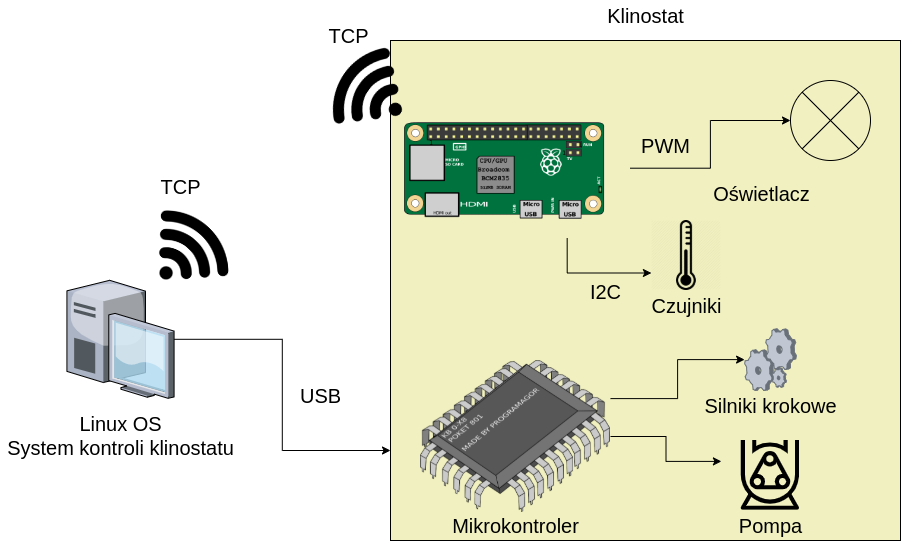
\includegraphics[scale=.4]{schemat_blokowy}
	\caption{Schemat blokowy systemu. Źródło: [opracowanie własne], PRZEROBIĆ TO, BO RPI JEST Z NIEZNANEGO ŹRÓDŁA I KOMPUTER POWINIEN BYĆ RDZEŃ SYSTEMU KONTROLI}
	\label{fig:schemat_blokowy}
	
\end{figure}